\subsubsection{Interrupts from the Pushbutton Keys}

Figure \ref{fig:pushbutton_port}, reproduced as Figure \ref{fig:pushbutton_port_int},
shows the registers associated with the pushbutton parallel port. 
The {\it Interruptmask} register allows interrupts to be generated when a key is
pressed.  Each bit in the {\it Edgecapture} register is set to 1 by the parallel port when the
corresponding key is pressed. An interrupt service routine can read this register
to determine which key has been pressed.  Writing any value to the
{\it Edgecapture} register deasserts the interrupt signal being sent to the
\GIC~and sets all bits of the {\it Edgecapture} register to zero.

\begin{figure}[h!]
   \begin{center}
       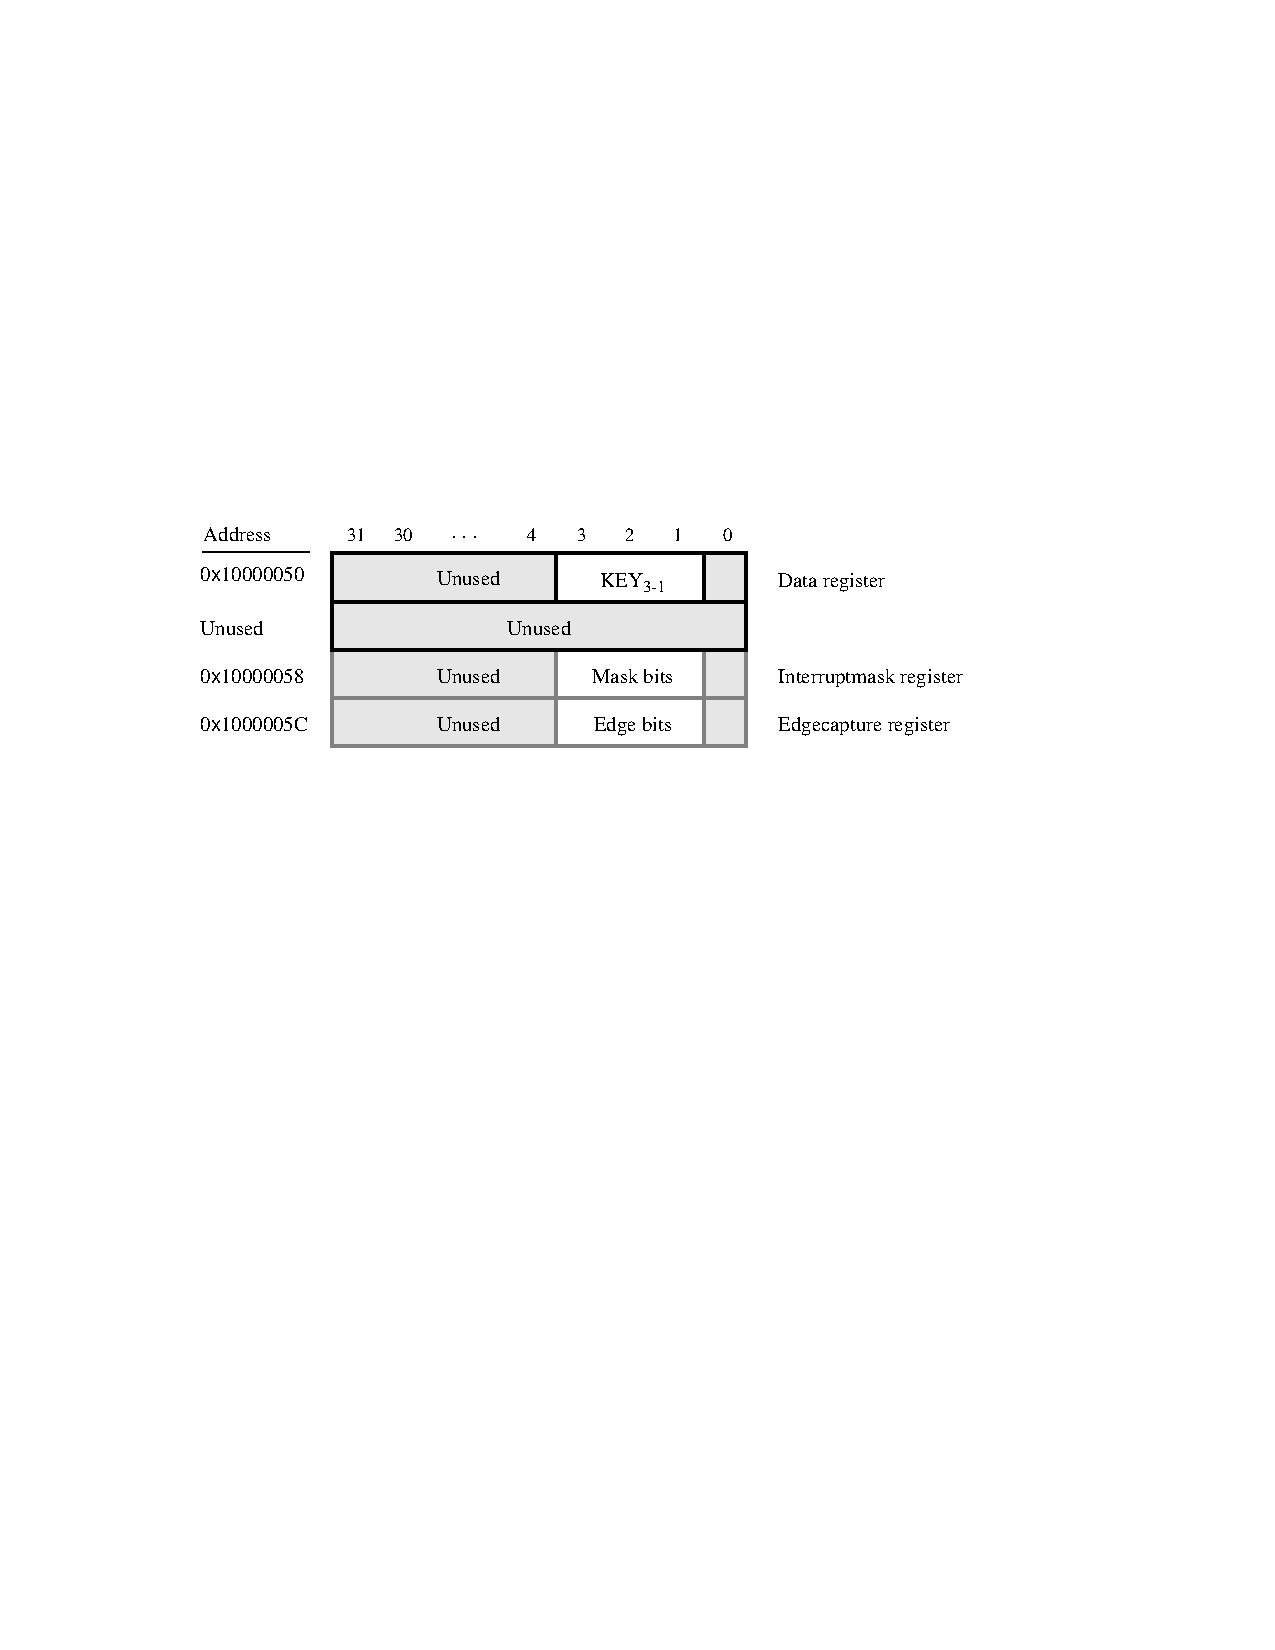
\includegraphics{../../../common/figs/FPGA_PP_Keys_3.pdf}
   \end{center}
   \caption{Registers used for interrupts from the pushbutton parallel port.}
	\label{fig:pushbutton_port_int}
\end{figure}

